\section{Actividad 7}

\subsection*{En la Fig. \ref{fig:diagrama} podrá observar el diagrama en bloques simplificado de un receptor de televisión satelital 
(similar a los que se encuentran en centros de distribución CATVCommunity Antenna Television). La temperatura de ruido antena-línea 
de alimentación es 50 K. Calcular la temperatura equivalente de ruido del sistema.}

    \begin{figure}[H]
            \centering
            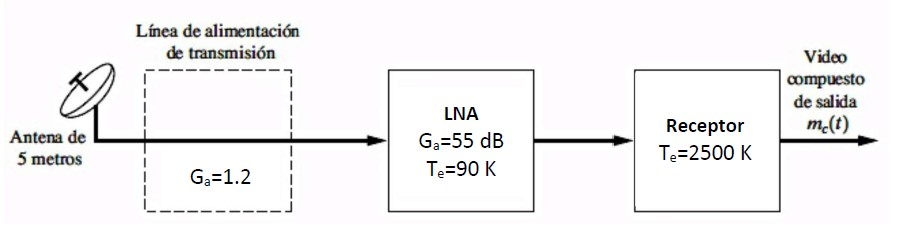
\includegraphics[width=0.8\linewidth]{imagenes/Actividad_7/actividad_7.jpg}
            \caption{Diagrama en bloques.}
            \label{fig:diagrama}
    \end{figure}

    Utilizando la fórmula de Friis, la cual permite expresar la temperatura de ruido equivalente de un sistema compuesto por varias etapas en función de las 
    temperaturas de ruido y ganancias de cada etapa, se tiene que:
        
        \[
            T_{eq} = T_1 + \frac{T_2}{G_1} + \frac{T_3}{G_1 G_2} + \cdots           
        \]
    
    Para proceder con los calculos se necesita convertir las ganancias de dB a unidades lineales utilizando la fórmula:
    
        \[
            G_{linear} = 10^{\frac{G_{dB}}{10}}
        \]
    
    Al realizar las conversiones requeridas se obtienen los siguientes valores:
        \begin{itemize}
            \item $G_1 = 1,2$
            \item $G_2 = 316227,766$
        \end{itemize}

    Ahora, se sustituyen los valores conocidos en la fórmula de Friis:
        \[
            T_{eq} = 50 k + \frac{900 k }{1,2} + \frac{2500 k }{1,2 \times 316227,766} = 125,0088 k
        \]

    Por lo tanto, la temperatura equivalente de ruido del sistema es igual a $125,0088 K$.
